\documentclass[output=paper]{LSP/langsci} 
\author{Oliver Čulo\and 
Silvia Hansen-Schirra\and 
Karin Maksymski\affiliation{Universität Mainz, Germersheim}\lastand Stella Neumann\affiliation{IFAAR, RWTH Aachen}
}
\title{Empty links and crossing lines: Querying multi-layer annotation and alignment in parallel corpora} 
\abstract{Translation shifts can be informative in various ways. Amongst other things, they can point to typological differences between languages or be indicators of properties of translated text like explicitation or normalisation. Detecting translation shifts in parallel corpora is thus a major task from the viewpoint of translation studies. This paper presents an analysis of translation shifts in a parallel corpus (English-German). It offers an operationalisation of queries which can exploit multi-layer annotation and alignment in order to detect various kinds of translation shifts across category boundary lines and empty alignment links. The paper furthermore discusses the shifts and links them to certain translation properties.}
\maketitle

\begin{document}
\shorttitlerunninghead{Empty links and crossing lines}
\lehead{Čulo, Hansen-Schirra, Maksymski \& Neumann}
%culo@uni-mainz.de, hansenss@uni-mainz.de, maksymsk@uni-mainz.de
%st.neumann@mx.uni-saarland.de


%Keywords: parallel corpora, multi-layer annotation and alignment, corpus query, translation studies, translation shifts, translation properties


\section{Introduction}\label{sec:culo:1}

In both translation studies and contrastive linguistics, multilingual corpora have recently been used to study translation phenomena, i.e. translation shifts or translation properties (as proposed by \citealt{Baker1993, Baker1995, Toury1995}), as well as contrastive differences between languages. One such corpus is the English-German CroCo corpus \citep{Hansen-SchirraEtAlfc}. The corpus contains English and German originals and their translations into German and English, respectively. It can thus be used both as a comparable and a parallel corpus, e.g. to study contrastive differences (e.g. \citealt{Steiner2008}), translation phenomena (e.g. \citealt{CuloEtAl2008,Hansen-SchirraEtAl2007}) or register variation \citep{Neumann2008}. The corpus draws much of its potential from its multi-level stand-off annotation and alignment \citep{Hansen-SchirraEtAl2006}.

In this paper, we present a study based on the parallel data in the corpus, exploiting the multi-level alignment in order to detect translation phenomena. We show how the annotation and alignment of linguistic structures can help detect translation phenomena and provide data for their deeper analysis and interpretation. We demonstrate this by presenting data on and interpretations of so-called `empty links' and `crossing lines', two phenomena which we characterize in \sectref{sec:culo:2}.

In \sectref{sec:culo:3}, we briefly outline the technical background of this study, i.e. the structure of the corpus, the application programmer interface (API) for it and how the corpus was queried. In \sectref{sec:culo:4}, we discuss the results and possible interpretations of the queries with respect to certain grammatical levels. In \sectref{sec:culo:5}, we give an overview of possible future directions. 

\section{Empty links and crossing lines}\label{sec:culo:2}

Approaching translation from a naive perspective, all translation units should match corresponding units in the source texts, both in semantics and in grammatical analysis \citep{Padó2007}. This is, of course, unrealistic, not only because languages diverge, but also because translators make individual decisions. Very broadly speaking, originals and their translations therefore diverge in two respects. Units in the target text may not have matches in the source text and vice versa; thus no connection can be drawn and we speak of \textit{empty links}. Units which do have a counterpart with which they are aligned may be embedded in higher units which are not aligned, resulting in \textit{crossing lines}. This is, for instance, the case when a word is embedded in a chunk with the subject function in one language, and its counterpart in a chunk with the object function.\footnote{The term \textit{crossing line} does not refer to crossing edges in the alignment. The image behind the term is rather that some unit which is embedded in another unit does not follow the alignment path (if there is any) of the higher unit it is embedded in, but ``crosses a line'' and enters the realm of another unit.} These two concepts are related, on the one hand, to concepts used in formal syntax and semantics, like null elements and discontinuous constituency types in LFG \citep{Bresnan1982} or HPSG \citep{Pollard1994}. On the other hand, they are in the tradition of well-known concepts in translation studies such as one to zero correspondence and translation shifts (\citealt{Koller2001,Vinay1958,Catford1965,Newmark1988,Leuven-Zwart1989,Cyrus2006}, among others).


We analyze for instance stretches of text contained in one sentence in the source text but spread over two sentences in the target text, as this may have implications for the overall information contained in the target text. We would thus pose a query retrieving all instances where the alignment of the lower level is not parallel to the higher level alignment but points into another higher level unit. In the example below, the German source sequence (1a) as well as the English target sequence (1b) both consist of three sentences which are aligned to each another.

\ea\label{ex:culo:1}
    \ea \textit{Aus dem Augenwinkel sah ich, wie eine Schwester dem Bettnachbarn das Nachthemd   wechselte. Sie rieb den Rücken mit Franzbranntwein ein und massierte den etwas   jüngeren Mann, dessen Adern am ganzen Körper bläulich hervortraten. Ihre Hände   ließen ihn leise wimmern. \textup{(GO\_FICTION\_002)}}\\
    \ex \textit{Out of the corner of my eye I watched a nurse change his neighbor's nightshirt and rub   his back with alcoholic liniment. She massaged the slightly younger man, whose veins   stood out blue all over his body. He whimpered softly under her hands.}
    \z
\z

In German, the first sentence is subdivided into two clauses, the second one into three. The first English target sentence contains three clauses and the second sentence two. The third sentences in both versions are co-extensive with the clause contained in them. We can see in example \REF{ex:culo:1} that the German clause 3 (\textit{Sie rieb den Rücken mit Franzbranntwein ein}) in sentence 2 is part of the coordinated raising construction (\ldots\textit{and rub his back with alcoholic liniment}) in the English sentence 1. The alignment of this clause points out of the aligned first sentence, thus constituting a crossing line. 

The third sentence also contains a crossing line, this time at the levels of grammatical functions and word alignment: the words \textit{Ihre Hände} in the German subject are aligned with the words \textit{her hands} in the English adverbial. However, this sentence is particularly interesting in view of empty links as shown in \citet{Hansen-SchirraEtAl2006}. The empty links are marked by a black dot in \figref{fig:culo:1}.

\begin{figure}
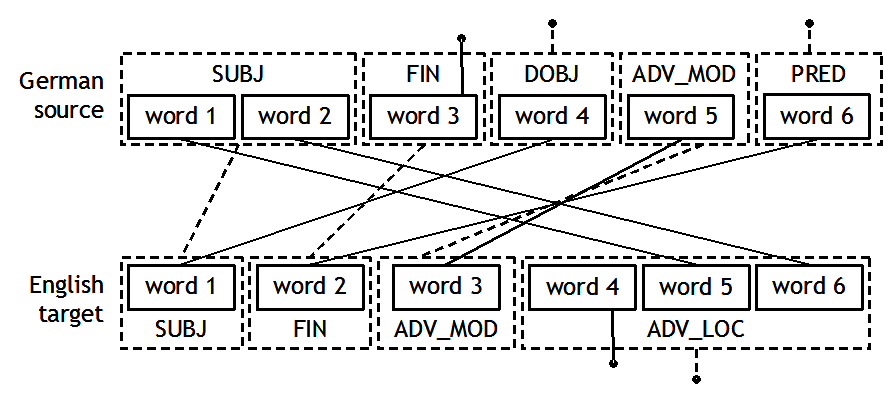
\includegraphics[width=\textwidth]{figures/CuloF1.png}
\caption{Alignment of grammatical functions and words in sentence 3}
\label{fig:culo:1}
\end{figure}

Our linguistic interpretation is based on a functional view of language. As explained in \sectref{sec:culo:3}, chunk alignment is based on the mapping of grammatical functions. Hence, the finite \textit{ließen} (word 3) in the German sentence is interpreted as a semi-auxiliary and thus as the finite part of the verbal group. Therefore, \textit{wimmern} (word 6) receives the label PRED (for predicator),\footnote{We are assuming in our annotation an analysis of the verb phrase into \textit{Finite} and \textit{Predicator} following \citealt[78ff]{halliday_introduction_1985}.} i.e. the non-finite part of the verb phrase, in the functional analysis. At word level, this German word is linked to word 2 \textit{(whimpered)} in the target sentence, which is assigned FIN, i.e. the finite verb in the layer of grammatical functions. As FIN exists both in the source and in the target sentences, this chunk is aligned. The German functional unit PRED does not have an equivalent in the target text and receives an empty link. Consequently, word 3 in the source sentence \textit{(ließen)} also receives an empty link. This mismatch will be interpreted in view of our translation-oriented research in \sectref{sec:culo:4}. In the following subsection we will see how these two phenomena can be retrieved automatically.

\section{Building and querying the corpus}\label{sec:culo:3}
\subsection{Corpus construction}\label{sec:culo:3.1}

The CroCo corpus consists of English originals (EO), their German translations (GTrans) as well as German originals (GO) and their English translations (ETrans). Both translation directions are represented in 8 registers, with at least 10 texts totaling 31,250 words per register. Altogether, the CroCo Corpus comprises approximately one million words. Additionally, register-neutral reference corpora are included for German and English, comprising 2,000 word samples from 17 registers.

The corpus thus consists of both a comparable and a parallel part. The registers are political essays (ESSAY), fictional texts (FICTION), instruction manuals (INSTR), popular-scientific texts (POPSCI), corporate communication (SHARE), prepared speeches (SPEECH), tourism leaflets (TOU) and websites (WEB). They were selected because of their relevance for the investigation of translation properties in the language pair English-German. All texts are annotated with

\begin{itemize}
\item 
meta information following the TEI standard \citep{Sperberg-McQueen1994, Burnard2007} including a brief register analysis that allows additional filter options, 
\item 
part-of-speech information using the TnT tagger \citep{Brants2000} with the STTS tag set for German \citep{SchillerEtAl1999} and the Susanne tag set for English \citep{Sampson1995},
\item 
morphology using MPRO \citep{Maas2009} which operates on both languages,
\item
grammatical functions of the highest nodes in the sentence, manually annotated with MMAX2 \citep{Müller2006}.
\end{itemize}

Furthermore, all texts are aligned on 

\begin{itemize}
\item  
word level using GIZA++ \citep{Och2003},
\item
chunk level (indirectly) by mapping the grammatical functions onto each other,
\item 
clause level (manually) again using MMAX2,
\item 
sentence level using the WinAlign component of the Trados Translator's Workbench \citep{Heyn1996} with additional manual correction.
\end{itemize}

The CroCo data are stored in an XML file format based on the corpus encoding standard XCES,\footnote{http://www.xces.org, last visited 3 December 2009} a multi-layer stand-off markup format. The CroCoXML format is described in detail in \citet{Hansen-SchirraEtAl2006,Hansen-Schirra2012}.

\subsection{CroCoAPI}\label{sec:culo:3.2}

Processing of corpus data -- annotation, querying and the like -- happens on various linguistic levels and usually involves different applications suited to one particular task (e.g. PoS tagging). Thus, the necessity often arises to convert corpus data into a certain, tool-dependent input format, and then back from the output format to the corpus format. Ideally, a corpus is embedded in some sort of larger framework which manages the data streams or even already comprises a number of applications working in some sort of processing pipeline.

In the case of the CroCo corpus, we created our own \textit{application programming interface} (API) to manage ever more complex queries, including queries operating on multiple annotation and alignment layers, and to apply Java-based annotation tools to the corpus data. The prerequisites for the API were:


\begin{itemize}
\item  
quick integration,
\item  
support of complex queries, also on alignment, 
\item  
no complex conversion into other formats required, and
\item  
possibly, integration of multiple formats.
\end{itemize}

The CroCoAPI presented here is a Java API which includes a light-weight, format-independent data structure that serves as communication interface to other applications. The following paragraphs describe the basic design of the API (Java classes and API layers are typeset in capitals.)

The API is made up of three parts. On top, there is the actual interface \textsc{CroCoIF}, the control methods of which present the basic read/write and iteration calls for the \textsc{CroCo} corpus data. Under the hood, a package called \textsc{CoReTool} is used to represent linguistic structures in stratified layers, and the parallel structures (e.g. aligned words, sentences, etc.) as sets of pairs. As an intermediate level, there is the CroCoXMLIO package, which handles the XCES-based CroCo data format. The CroCoIF communicates with CroCoXMLIO using the \textsc{CoReTool} data structures.

Fundamental within the API is the notion of \textsc{Text}. The \textsc{Corpus} is a collection of \textsc{Texts}, and each \textsc{Text} contains a thematically coherent set of linguistic structures. The list of available \textsc{Texts} can be generated for the whole corpus or per register, as singletons or as pairs of original and translation.

In the multi-layer layout of CroCo, linguistic units like sentences or chunks are defined on the basis of lists of tokens. There is no explicit information about the syntactic hierarchies, e.g. whether a certain chunk belongs to a certain sentence. However, for a number of applications it is helpful or even required to convert this representation into a stratificational structure as provided by \textsc{CoReTool.}

The \textsc{CoReTool} data structure was designed to be a format-neutral representation of the linguistic structures generally found in a corpus. The data structure is used within the CroCoAPI to communicate between the interface and the input-output (IO) level; it can, furthermore, be used as data connector to applications such as the lexical chainer embedded in DKPro (\citealt{GurevychEtAl2007}, see below). In general, one could enhance the CroCo corpus with various data formats and integrate these with \textsc{CoReTool}; this would only need additional read-/write-methods for handling the different data formats. This stratificational approach is a major difference between the CroCoAPI and other APIs like TigerAPI \citep{Özgür2007}, where programming data structures and underlying data format are more closely linked, and a conversion to TigerXML is necessary for a corpus before using it with any aspects of the TigerAPI.

\textsc{CoReTool} represents the linguistic data in stratified layers, following classical linguistic strata. This differs from the representation in CroCoIF, where all linguistic structures such as sentences or chunks are defined on the basis of tokens. 

A \textsc{Corpus} is made up of an ordered collection of \textsc{Texts}, which again is made up of an ordered collection of \textsc{Sentences}, which again is made up of an ordered collection of \textsc{Tokens}. This structure is, so to speak, the backbone of \textsc{CoReTool} and the minimum of data that we expect in a corpus. In addition, a \textsc{Corpus} can be divided into \textsc{Registers} which also relate to collections of \textsc{Texts} (from the \textsc{Corpus}). Likewise, a \textsc{Sentence} can contain \textsc{Clauses} or \textsc{Chunks} which relate to the \textsc{Tokens} of the \textsc{Sentence}. For each of these subunits of a text (including \textsc{Tokens}), it is possible to have aligned counterparts. Every single alignment is represented as a pair; so if unit \textit{U} is aligned with \textit{U'} and \textit{U''}, there will be two pairs <\textit{U},\textit{U'}> and <\textit{U},\textit{U''}>.

The \textsc{CoReTool} Java package uses simple data structures like ordered lists to organize the linguistic content it represents. In addition, a couple of basic methods for calculating statistics -- e.g. the number of chunk types -- are included. The package so far lacks a proper backend-enabled design, so that IO methods could be plugged in on demand. Also, the linguistic representation of \textsc{CoReTool} is currently restricted to syntactic structures.

\subsection{Querying the aligned corpus}\label{sec:culo:3.3}

In CroCoXML, the alignment is stored in one XML file per level. Alignments between words are, for instance, represented as follows:

\ea
\begin{lstlisting}
<word>
    <align xlink:href="#t3076"/>
    <align xlink:href="#t3301"/>
</word>
<word>
    <align xlink:href="#t3077"/>
    <align xlink:href="#undefined"/>
</word> 
\end{lstlisting}
 \z


In the pairs of words, the first entry relates to the source text word and the second to the target text word. For the word alignment, we decided to explicitly state empty links by including an element \textit{\#undefined} where no corresponding word exists for a source or target language token, which we can read off from the automatic alignment data. This is not the case for the clause or sentence alignment, which was done, or at least corrected, manually.

For the queries on empty links on word level, it would be sufficient to evaluate the XML alignment. A simple way to query for empty links would have been to query the XML annotation for pairs where one element is \textit{\#undefined}. However, the implementation results in more abstract ways to query the data. The alignment is read in from the XML files and packed into abstract data structures, representing tokens and token pairs (i.e. aligned tokens), clauses and clause pairs, etc. These abstract data structures are passed on to a query processor. This design allows both for the simple empty link queries and for the more complex crossing line queries. Also, this adheres to our aim of keeping the processing of the corpus format and the processing on linguistic structures separate.\footnote{Partly, the queries are realized on the format-independent CoReTool level. For the most part, however, the queries still use the proprietary CroCoXML API, because the API was still in development at the time of writing and not all levels had been sufficiently and transparently  distinguished from one another.}

Applied to the parallel sentence from the empty link example in \sectref{sec:culo:2}, the empty link query returns all German original words which receive an empty link due to a missing equivalent in alignment (in this case \textit{ließen}). The same query can also be applied to the other alignment layers: see \sectref{sec:culo:4.1} for empty links at the level of grammatical functions and \sectref{sec:culo:4.2} for empty links at clause level.

Querying crossing lines in the aligned source and target sentences combines the alignment on two levels, e.g. word level and the mapping of grammatical functions. Crossing lines are identified, for instance at this level, by querying for words in one grammatical function in one language which are aligned with words in a different grammatical function in the other language. An example algorithm (pseudo-code) is given in \REF{ex:culo:pseudocode}.

% \begin{figure}
\ea
\begin{lstlisting}
for every word_pair in word_pairs 
  sl_clause : = 
    get_clause(get_sl_word(word_pair)) 
  tl_clause : = 
    get_clause(get_tl_word(word_pair)) 
  is_aligned?(sl_clause, tl_clause) 
end 
\end{lstlisting}
% \caption{Pseudo-code for a query on crossing lines between words and clauses}
\label{ex:culo:pseudocode}
\z
% \end{figure}

Applying the query to example \REF{ex:culo:1} returns the German words \textit{Ihre Hände}, which are part of the German subject and which are aligned with the English words \textit{her hands}, which are part of the second adverbial. The query for crossing lines between words and grammatical functions is different from other queries, as there is no explicit chunk alignment. When querying for crossing lines between words and clauses, we can make use of the data from the manual clause alignment. Additionally, other alignment layers may be investigated with similar queries, e.g. crossing lines between grammatical functions and clauses.\footnote{It should be noted that precision and recall of the query results can only be as accurate as the word alignment provided by GIZA++ (cf. \citealt{CuloEtAl2008}). This limits the validity of the query results for crossing lines and empty links on all levels involving word alignment.}

\section{Some selected phenomena}\label{sec:culo:4}

In this section, we will discuss empty links with respect to grammatical functions (\sectref{sec:culo:4.1}) and clauses (\sectref{sec:culo:4.2}) as well as crossing lines for words and grammatical functions (\sectref{sec:culo:4.3}). The three aspects were chosen because they represent a range of queries as well as translation phenomena. The discussion concentrates on the three registers FICTION, SHARE and SPEECH, which show a sufficient range of variation to detect registerial influences on translation properties. 

\subsection{Empty links at the level of grammatical functions}\label{sec:culo:4.1}

At the level of grammatical functions, the following tendencies in connection with empty links, i.e. non-aligned segments, can be identified. As \figref{fig:culo:grammaticalfunction} shows, percentages for empty links in the translation direction English-German are rather similar for originals and translations, with SHARE exhibiting a slightly higher percentage of unmapped functions for the German translations. When looking at the translations from German to English, however, there is a clear tendency for German texts to exhibit more unmapped functions than the English translations. 

\begin{figure}
\begin{tikzpicture}
\pgfplotstableread{ % Read the data into a table macro
% table rows are listed upside down here as
% the algorithm seems to process rows last-in-first-out
Label   Aligned   NotAligned
ETrans\_SPEECH	94.41	5.59
GO\_SPEECH	85.74	14.26
ETrans\_SHARE	93.14	6.86
GO\_SHARE	77.83	22.17
ETrans\_FICTION	91.8	8.2
GO\_FICTION	78.19	21.81
GTrans\_SPEECH	93.8	6.2
EO\_SPEECH	85.66	14.34
GTrans\_SHARE	91.38	8.62
EO\_SHARE	85.18	14.82
GTrans\_FICTION	88.82	11.18
EO\_FICTION	78.85	21.15
}\datatable

\begin{axis}[
    xbar stacked,   % Stacked horizontal bars
    xmin=0, xmax=100,        % Start x axis at 0
    xlabel={Percentage (\%)},
    ytick=data,     % Use as many tick labels as y coordinates
    yticklabels from table={\datatable}{Label},  % Get the labels from the Label column of the \datatable
    legend style={
            at={(.2,.01)},
            anchor=south
         	}
]

\addplot [fill=lsMidBlue] table [x=Aligned, y expr=\coordindex] {\datatable};    % Plot the "First" column against the data index
\addplot [fill=lsDarkBlue]table [x=NotAligned, y expr=\coordindex] {\datatable};
%\addplot [fill=red!80!yellow] table [x=Third, y expr=\coordindex] {\datatable};
\legend{Aligned,NotAligned}

\end{axis}

\end{tikzpicture}

\caption{Statistics for alignment of grammatical function}
\label{fig:culo:grammaticalfunction}
\end{figure}

We have chosen the English-German SHARE texts for a closer look at the distribution of empty links for grammatical functions. \tabref{tab:culo:1} shows the percentage of empty links for the different grammatical functions in EO\_SHARE and GTrans\_SHARE. Empty links occur with different grammatical functions comparing English and German. The English originals, for example, have more empty links for appositions (APPO) and complements (COMPL), but fewer empty links for predicators (PRED) or modal adverbials (ADVmod). This means that the English original appositions and complements tend to be realized differently in the German translations. Furthermore, the German translated predicators and modal adverbials tend to have other realizations in the source language texts. These differences might be a sign of implicitation or explicitation effects (cf. 
\citealt{Hansen-SchirraEtAl2007}). They might, however, also be explained through translation shifts on the level of grammatical functions.

\begin{table}
\resizebox{\textwidth}{!}{
\begin{tabular}{lrrr}
\lsptoprule
Tag & Explanation & EO-SHARE & GTrans-SHARE\\
\midrule
ADV\_CAUSE & causal adverbial (\textit{therefore}) &  4.00 & 0.83\\
ADV\_LOC & locative (\textit{in the house}) & 3.72 & 2.76\\
ADV\_MOD &  modal adverbial (\textit{with pleasure}) & 4.65 &  12.02\\
ADV\_TEMP &  temporal adverbial (\textit{yesterday}) &  3.16 &  4.97\\
ADV\_OTHER & other adverbials (\textit{however}) &  3.53 & 4.01\\
APPO & apposition (\textit{\ldots, }\textit{which makes no sense}) & 7.07 &  0.14\\
COMPL & complement (\textit{He is }\textit{a teacher}) &  18.51 & 1.66\\
CONJ & sentence-initial conjunction (\textit{but}) & 7.81 & 12.85\\
DOBJ & direct object (\textit{I hit }\textit{the ball}) & 16.19 &  11.05\\
FIN &  finite part of the verb (\textit{has}\textit{ seen}) &  0.19 & 0.69\\
IOBJ & indirect object (\textit{Tell }\textit{him}) & 2.51 &  4.97\\
NEG &  sentence negation (\textit{We did}\textit{n't}\textit{ go}) &  1.12 &  0.83\\
MINOR &  verbless sentence (\textit{Dear customers!}\textit{)} &  1.3 &  0.69\\
PART & particle (\textit{It was }\textit{just}\textit{ funny}) &  2.79 & 10.91\\
PRED &  non-finite part of verb (\textit{has }\textit{seen}) &  14.6 & 30.11\\
PROBJ & prepositional object (\textit{rely }\textit{on s.o.}) &  8.19 & 0.55\\
SUBJ & subject (\textit{She}\textit{ is a doctor}) &  0.65 & 0.97\\
\lspbottomrule
\end{tabular}
}
\caption{Distribution of empty links for grammatical functions (in \%)}
\label{tab:culo:1}
\end{table}

The following examples illustrate the observation that the frequency of empty links for appositions is higher in the English original SHARE texts than in the German translations.

\newpage 
In example \REF{ex:culo:2} the English apposition \textit{a record} is an interpretation of the facts presented in this sentence. Example \REF{ex:culo:3} exhibits a very similar rhetorical move in the apposition \textit{an improvement of 2.3 turns}. In both cases, the appositions are translated by coordinated finite sentences -- in the latter one even in inverse order -- thus adding linguistic information by spelling out implicit information (cf. \citealt{Hansen-SchirraEtAl2007} for more discussion of such phenomena). Obviously, this is one of the sources of empty links between source and target segments.

\ea\label{ex:culo:2}
   \ea 
    \textit{Revenues rose 11\% to \$112 billion, a record. \textup{(EO\_SHARE\_004)}}\\
    \ex \textit{Der weltweite Umsatz stieg um 11\% auf \$112 Mrd. und erreichte damit eine neue Rekordhöhe. \textup{(GTrans\_SHARE\_004)}} 
   \z
\z


\ea \label{ex:culo:3} 
   \ea \textit{Working capital turns hit an all-time high of 11.5 - an improvement of 2.3 turns. \textup{(EO\_SHARE\_004)}} \\
    \ex \textit{Die Umschlagshäufigkeit des Betriebskapitals konnte um das 2,3 fache gesteigert   werden und erreichte die neue Höchstmarke von 11,5. \textup{(GTrans\_SHARE\_004)}}
     \z
\z


The high frequency of empty links for complements may be due to registerial and typological constraints of the English SHARE texts. Example \REF{ex:culo:4} shows that the English verb \textit{name} is followed by a complement, whereas the German verb \textit{ernannte} is followed by a prepositional object. This is, of course, an obligatory shift due to typological differences between the languages. However, the frequent use of these constructions might be attributed to the register on the basis of a combined interpretation of verb semantics and valency. A possible explanation could then be that companies are supposed to distinguish themselves from other companies and enumerate their achievements. Example \REF{ex:culo:5} again illustrates typological differences between English and German. Whereas English uses a subject complement in the construction \textit{We are pleased}\ldots, the German translation is realized by the finite reflexive verb \textit{(sich) freuen}, but no subject complement, and it is this non-mapping on the level of grammatical functions which creates the empty link here. In terms of ``markedness'', the original construction is typical of English, just as the translated construction is typical of German, thus explaining the number of empty links for English complements.


\ea \label{ex:culo:4}
   \ea \textit{Also for the second straight year, we were named ``The World's Most Respected Company'' by the Financial Times.} (EO\_SHARE\_004) \\
   \ex 
   \textit{Ebenfalls zum zweiten Mal in Folge ernannte die Financial Times GE zum `` am meisten respektierten Unternehmen der Welt''.} (GTrans\_SHARE\_004)
   \z
\z
 
 
\ea \label{ex:culo:5}
  \ea \textit{We are pleased to present the 2001 Annual Report of the American Institute for   Contemporary German Studies (AICGS). \textup{(EO\_SHARE\_013)}}\\
   \ex \textit{Wir freuen uns, Ihnen den Jahresbericht 2001 des American Institute for Contemporary   German Studies (AICGS) präsentieren zu können.} (GTrans\_SHARE\_013) 
   \z
\z

The high frequency of empty links for predicators in the German translations is due in most cases to typological and register constraints: example \REF{ex:culo:6} illustrates a shift in tense which involves using the predicator, i.e. the non-finite part of the verb phrase \textit{geschafft}. In examples \REF{ex:culo:7} and \REF{ex:culo:8} the English active constructions are translated by passives in German, which include the predicators, the past participles \textit{beschrieben} and \textit{weiterentwickelt}. The choice of passive is motivated by the register since this German specialized register tends to favour a content-oriented style expressed by dense noun phrases as well as passivization (cf. \citealt{Neumann2008}). Here, typical structures of the target language register are chosen by the translators. 

\ea \label{ex:culo:6}
  \ea  \textit{We already have that! \textup{(EO\_SHARE\_004)}}\\
   \ex \textit{Das alles haben wir bereits geschafft. \textup{(GTrans\_SHARE\_004)}}
   \z
\z


\ea \label{ex:culo:7}
  \ea \textit{In that report, we described several challenges and opportunities that we felt were   going to determine the agenda of German-American relations. \textup{(EO\_SHARE\_013)}} \\
   \ex \textit{In diesem Bericht werden verschiedene Herausforderungen und Gelegenheiten beschrieben, die unserer Meinung nach die Beziehungen der beiden Staaten bestimmen. \textup{(GTrans\_SHARE\_013)}}
   \z
\z


\ea \label{ex:culo:8}
   \ea \textit{It progresses with a drumbeat regularity throughout our business year - year after year. \textup{(EO\_SHARE\_004)}}\\
    \ex \textit{Jahr für Jahr wird das Betriebssystem mit der Regelmäßigkeit eines Paukenschlages weiterentwickelt.} \textup{(GTrans\_SHARE\_004)} 
    \z
\z

The reasons for finding more empty links for modal adverbials in the German translations seem to be manifold: example \REF{ex:culo:9} shows an added modal adverbial in the target language text. The back-translation of the German target text reads: \textit{Wireless networks will change the workplace fundamentally}. The English word \textit{transform} is translated through the weaker German verb \textit{verändern} `change' in combination with the modal adverb \textit{grundlegend} `fundamentally'. This can be interpreted as a more explicit German version of the English verbal construction.\footnote{Cf. \citet{Hansen-SchirraEtAl2007} for a discussion of explicitation vs. addition.} Concerning the modal adverbial \textit{persönlich} (\textit{face-to-face}) in example \REF{ex:culo:10}, implicit information in the source text is rendered explicit in the translation. In both cases, however, the translators probably try to emphasize relevant information, thus making the text easier or faster to understand. Example \REF{ex:culo:11} illustrates a case of typologically-driven translation behavior: the English raising construction \textit{continue to benefit} is not available in German (cf. \citealt[75ff]{Hawkins1986}). Therefore, the translator chose a different lexico-grammatical realization (i.e. the addition of an adverbial), adapting the German translation to target language norms.


\ea \label{ex:culo:9}
   \ea  \textit{Wireless networks will transform the workplace. \textup{(EO\_SHARE\_005)}}\\
   \ex \textit{Drahtlose Netzwerke werden den Arbeitsplatz grundlegend verändern. \textup{(GTrans\_SHARE\_005)}}
    \z
\z 


\ea \label{ex:culo:10} 
   \ea \textit{Mostly, it involves creating and distributing paper documents or telephoning and meeting with fellow employees. \textup{(EO\_SHARE\_005)}}\\
  \ex \textit{In den meisten Fällen erstellen und verteilen sie Papierdokumente oder telefonieren   oder treffen sich persönlich mit anderen Mitarbeitern. \textup{(GTrans\_SHARE\_005)}}
  \z
\z


\ea \label{ex:culo:11}
   \ea
 We continue to benefit from the strong natural gas market in North America. \textup{(EO\_SHARE\_002)}
   \ex 
   Wir profitieren weiterhin von einem starken Erdgasmarkt in Nordamerika. \textup{(GTrans\_SHARE\_002)}
   \z
\z


In summary, empty links on the level of grammatical functions show some interesting and varied patterns. Some of the empty links may be attributed to different usage patterns, for instance in the case of English complements and German prepositional objects. Others are due to more general contrastive differences such as the (non-)availability of raising constructions in one of the languages, or different kinds of constraints on the mapping from semantic roles to grammatical functions. A more in-depth inspection of all hits for the query could provide an interesting overview of translation properties on this layer.

\subsection{Empty links at clause level}\label{sec:culo:4.2}

For the distribution of empty links at clause level another general tendency can be observed. At clause level, it seems to be a clear characteristic of the English texts to exhibit more empty links. All English original texts as well as all English translations have more empty links than their matching German texts (see \figref{fig:culo:clausealignment}), with English translations in SPEECH displaying the highest number: here, 35\% of the clauses have no link to a clause in the German source text. 

When correlating the number of empty links with the total number of clauses, we find a similar picture. In SPEECH as well as in the other registers, the English texts always display a higher number of clauses, although all corpora are of approximately the same size in terms of number of words. Here it is important to bear the following point in mind: the clause segmentation in CroCo is verb-based, i.e. each verb (finite or non-finite) is taken as the basis of a new clause. Thus, empty links occur where a clause (containing a verb) in one text has no direct verbal equivalent in the respective text of the other language either because the content of this clause is expressed in a non-verbal construction or because it is simply left out.

For the register SPEECH, the numbers are as displayed in \tabref{tab:culo:2}.

\begin{table}
\begin{tabular}{lrrr} 
\lsptoprule
{} & total number clauses & aligned clauses & empty links\\
\midrule
GO\_SPEECH & 3,798 & 3,058 (80.52\%) & 740 (19.48\%)\\
ETrans\_SPEECH & 4,856 & 3,144 (64.74\%) & 1,712 (35.26\%)\\
EO\_SPEECH & 3,853 & 3,083 (80.02\%) & 770 (19.98\%)\\
GTrans\_SPEECH & 3,170 & 2,981 (94.04\%) & 189 (5.96\%)\\
\lspbottomrule
\end{tabular}
\caption{Clause alignment in SPEECH}
\label{tab:culo:2}
\end{table}

\begin{figure}
\begin{tikzpicture}
\pgfplotstableread{ % Read the data into a table macro
% table rows are listed upside down here as
% the algorithm seems to process rows last-in-first-out
Label   Aligned   NotAligned
ETrans\_SPEECH	64.74	35.26
GO\_SPEECH	80.52	19.48
ETrans\_SHARE	73.82	26.18
GO\_SHARE	91.23	8.77
ETrans\_FICTION	84.74	15.26
GO\_FICTION	92.98	7.02
GTrans\_SPEECH	94.04	5.96
EO\_SPEECH	80.02	19.98
GTrans\_SHARE	89.18	10.82
EO\_SHARE	77.64	22.36
GTrans\_FICTION	89.59	10.41
EO\_FICTION	86.65	13.35
}\datatable

\begin{axis}[
    xbar stacked,   % Stacked horizontal bars
    xmin=0, xmax=100,        % Start x axis at 0
    xlabel={Percentage (\%)},
    ytick=data,     % Use as many tick labels as y coordinates
    yticklabels from table={\datatable}{Label},  % Get the labels from the Label column of the \datatable
    legend style={
            at={(.2,.01)},
            anchor=south
         	}
]

\addplot [fill=lsMidBlue] table [x=Aligned, y expr=\coordindex] {\datatable};    % Plot the "First" column against the data index
\addplot [fill=lsDarkBlue]table [x=NotAligned, y expr=\coordindex] {\datatable};
%\addplot [fill=red!80!yellow] table [x=Third, y expr=\coordindex] {\datatable};
\legend{Aligned,NotAligned}

\end{axis}

\end{tikzpicture}

\caption{Clause alignment statistics}
\label{fig:culo:clausealignment}
\end{figure}




The numbers in the second column (aligned clauses) probably represent unproblematic cases, where clauses in the source text can easily be connected to clauses in the target text, perhaps due to similar constructions or rather simple sentences. 

The figures in the third column (empty links) leave room for interpretation. Concerning the translation direction German-English, we find that in many cases empty links occur in English subordinate clauses or expressions that resolve more complex structures of the German original text. These are, for example, nominalizations or nouns with premodifying participle constructions, as can be seen in \REF{ex:culo:12} and \REF{ex:culo:13}.


\ea \label{ex:culo:12}
  \ea \textit{[Mittlerweile ist anerkannt,] [dass es zur Sicherung von Beschäftigung vor allem auf   Flexibilität ankommt.] \textup{(GO\_SPEECH\_007)}}\\
  
\newpage 
    \ex \textit{[It has now been recognized] [that flexibility is the most important factor] [when it comes] [to safeguarding jobs.] \textup{(ETrans\_SPEECH\_007)}}
    \z
\z 

\ea \label{ex:culo:13}
   \ea \textit{[Die Staats- und Regierungschefs der Europäischen Union haben in Göteborg erneut   ihre Bereitschaft bekräftigt,] [die in Kyoto eingegangenen Verpflichtungen zur   Verminderung der Treibhausgase zu erfüllen.] \textup{(GO\_SPEECH\_001)}}\\
   \ex \textit{[In Gothenburg the EU heads of state and government reaffirmed their willingness] [to fulfil the commitments] [they made in Kyoto] [to reduce greenhouse gases.] \textup{(ETrans\_SPEECH\_001)}}
   \z
\z

In both examples, there are only two clauses in the German sentence; these are split into four and three clauses in the respective English translations.\footnote{Clauses are segmented irrespective of their dependence within the syntactic structure. Therefore, embedding cannot be retraced.} In \REF{ex:culo:12}, the nominal group \textit{zur Sicherung von Beschäftigung} is transformed into two subordinate clauses with a finite verb (\textit{comes to}) and a non-finite one (\textit{safeguarding}). In \REF{ex:culo:13}, the participle of the nominal group \textit{die in Kyoto }\textit{eingegangenen}\textit{Verpflichtungen} is translated with the finite verb \textit{made}. This strategy results in one more clause in the English translation than in the German original and therefore in an empty link for this additional clause. There seems to be a tendency within the English translations to use formulations that are more explicit and less dense than those in the German texts. \citet{Fabricius-Hansen1998} reports similar results in a comparison of German source texts and the respective translations into English and Norwegian and discusses a ``tendency towards higher informational density that can be observed in German texts of the relevant type and which is correlated with a relatively high degree of syntactic complexity'' \citep[197]{Fabricius-Hansen1998}. She relates this phenomenon to different types of discourse information structure, assigning a ``hierarchical type'' to German texts and an ``incremental'' one to the English translations \citep[202--203]{Fabricius-Hansen1998}, with the latter increasing incrementality by information splitting \citep[231]{Fabricius-Hansen1998}. In terms of translation properties we could speak of simplification and explicitation here, i.e. a tendency in translations to simplify their texts and to spell things out rather than leaving them implicit \citep[180-181]{Baker1996}. At the same time, the high number of clauses can be interpreted as normalization: the translation (over-)uses typical features of the target language, such as a low informational density \citep[183]{Baker1996}.

Another example where the English translation shows a strong preference for verbal (especially non-finite) instead of nominal constructions is \REF{ex:culo:14}, which consists of one single clause in German and of four clauses in English. In the English sentence, the segments form one discontinuous clause with several embedded clauses in between, as marked by the brackets: 


\ea \label{ex:culo:14}
  \ea \textit{[Mit der am 16. Juli in Bonn beginnenden Klimakonferenz der Vereinten Nationen gehen die jahrelangen Bemühungen um ein verbindliches Klimaschutz-Abkommen in die entscheidende Phase.] \textup{(GO\_SPEECH\_001)}}\\
   \ex \textit{[With the UN Climate Conference [beginning in Bonn on July 16] the many years of efforts [aimed at] [achieving a climate protection agreement] will enter the crucial final phase.] \textup{(ETrans\_SPEECH\_001)}}
   \z
\z

Here, the German nominal expression \textit{Bemühungen um} is translated with \textit{efforts aimed at achieving}. The decision of the translator to use this construction results in two more clauses in the English sentence: instead of translating the German expression rather literally with \textit{efforts toward}, a longer and more explicit phrasing is used. Again, different types of information structure (hierarchical vs. incremental type, see above) could offer an explanation for the higher number of empty links in the English texts. Additionally, this example illustrates a further reason: the restricted options of English concerning pre- and postmodifying. In the German sentence, the noun \textit{Klimakonferenz} is premodified with the construction \textit{mit der am 16. Juli in Bonn beginnenden}. Since the participle \textit{beginnenden} is used in an adjectival way (as is almost always the case with premodifying participles) it does not form the basis of a new clause. The same information could have been conveyed using a less dense construction, e.g. a postmodifying relative clause like \textit{Mit der Klimakonferenz, die am 16. Juli in Bonn begann}, in this way splitting the sentence into two clauses. For English, all options to translate this sequence result in a postmodifying construction containing a verb. 


A considerable number of empty links in the English texts is due to properties of the language system that contrast with German. Here again a connection can be drawn to the translation property of normalization: \citet[218]{Teich2003} relates this to contrastive differences in the range of options available in source and target language, positing that fewer options in the target language entail compensations which may then lead to normalization. English has fewer options compared to German with respect to pre- and postmodification, which leads to normalization. That in turn would explain at least in part the high number of empty links. 

\newpage 
Still another explanation could be different registerial restrictions. In example \REF{ex:culo:15}, the German adverb \textit{deshalb} is translated with the expression \textit{that is why}, again resulting in an additional clause in the English text: 


\ea \label{ex:culo:15}
   \ea \textit{[Deshalb machen hohe Abgaben Arbeit teuer] [und können doch nicht verhindern,]   [dass unseren Sozialsystemen der Kollaps droht.] \textup{(GO\_SPEECH\_007)}}\\
   \ex \textit{[That is why] [high taxes make work expensive] [and yet cannot protect our social system from] [impending collapse.] \textup{(ETrans\_SPEECH\_007)}}
   \z
\z

It is possible that the use of \textit{therefore} instead of \textit{that is why} would sound too formal for a speech or that a more explicit reference to the previous sentence has to be made. In any case, this is an example for a situation in which the individual decision of the translator influences the number of empty links. If this proves to be a typical pattern (all three occurrences of \textit{that is why}~are in fact translations of \textit{deshalb}), it can be interpreted as a possible sign of explicitation because it shows a ``rise in the level of cohesive explicitness'' \citep[19]{Blum-Kulka1986}. 

For the translation direction English-German in SPEECH the picture is a different one, with only 5.96\% of empty links in the target texts (GTrans\_SPEECH). These are mainly cases where the translator has to opt for a different translation because of lexical differences of the verb as in (16) or where s/he uses a German non-finite construction that results in an additional clause in \REF{ex:culo:17}:

\ea \label{ex:culo:16}
   \ea \textit{[One of President Bush's primary objectives in that meeting was] [to take a further step in our efforts] [to persuade President Putin] [to join us in] [creating a new strategic   framework for] [dealing with the security threats] [that we now face,] [while moving us   toward a cooperative relationship with Russia and away from the adversarial legacy of the Cold War.] \textup{(EO\_SPEECH\_003)}}\\
    \ex \textit{[Eines der vorrangigen Ziele von Präsident Bush bei diesem Treffen war es,] [einen   Schritt voranzukommen bei unseren Bemühungen,] [Präsident Putin zu überzeugen,] [mit uns gemeinsam einen neuen strategischen Rahmen für die Handhabung von   Sicherheitsbedrohungen zu schaffen,] [denen wir uns nun gegenübersehen,] [während wir gleichzeitig auf kooperative Beziehungen zu Russland hinarbeiten] [und die feindliche Gesinnung des Kalten Kriegs hinter uns lassen.] \textup{(GTrans\_SPEECH\_003)}}
    \z
\z

 
\newpage 
Here, it is semantically impossible to retain the structure \textit{moving us toward\ldots and away from} in the translation. Two different verbs have to be used and thus one clause in the English text is split into two clauses in the German translation.

\ea \label{ex:culo:17}
   \ea \textit{[Our European friends and allies share our concern about the need] [to accord recognition to surviving Holocaust victims within their lifetimes.] \textup{(EO\_SPEECH\_006)} }
    \ex \textit{[Unsere europäischen Freunde und Bündnispartner teilen unser Anliegen,] [den   überlebenden Holocaust-Opfern zu Lebzeiten Anerkennung zuteil werden] [zu lassen.] \textup{(GTrans\_SPEECH\_006)}}
    \z
\z

In \REF{ex:culo:17}, the translator uses an infinitive construction with the modifying verb \textit{lassen}, which leads to two verbs and therefore two clauses, where the English original formulation consists of only one clause. 

Apart from these few cases, the German translations adhere rather closely to the English source texts. 94.04\% of the clauses are aligned, and it seems as if the translators are trying to use the same structures in the German texts that can be found in the English ones. This could be interpreted as source language shining through, which is, as it were, the `counterpart' of normalization. Lexico-grammatical properties of the source language can be reflected in the target language as well, especially in areas where the target language is more flexible than the source language \citep[218]{Teich2003}. With regard to pre- and postmodification it is therefore possible that the German translations follow the pattern used in the English originals, because German is not confined to one specific option, but can afford to more or less copy the structures of the English text. This strategy would result in a lower number of empty links. 

Nevertheless, it has to be borne in mind that there are also empty links in the English source texts. They occur, for example, where English non-finite constructions are translated with the help of nominal constructions, as can be seen in example \REF{ex:culo:18}. 

\ea \label{ex:culo:18}
   \ea 
   \textit{[As a result: in the Middle East, countries are going back to the negotiating table,] [we have established a new relationship with Russia] [that promises] [to form the a [\textup{sic}] new framework of constructive arms control agreements,] [and we are openly   discussing the very real problems and the hard reality] [attached to the proliferation of   weapons of mass destruction.]} \textup{(EO\_SPEECH\_005)}\\
   \ex \textit{[Das Ergebnis hiervon ist: -- die Rückkehr der Länder im Nahen Osten an den Verhandlungstisch, -- der Aufbau neuer Beziehungen zu Russland, [die das Versprechen eines neuen Rahmens für konstruktive Rüstungskontrollabkommen bergen,] und -- eine offene Diskussion über die sehr realen Probleme und die harsche Wirklichkeit im   Zusammenhang mit der Verbreitung von Massenvernichtungswaffen.]}  (GTrans\_SPEECH\_005)
   \z
\z

The results of US President Bush's policies are listed with bullet points in the English source text. For each result the author starts with a new sentence, sometimes containing several clauses. In the German translation, each result is presented as a noun phrase containing no verbs. As explained above, this rather dense discourse information structure is characteristic of German. 

Empty links at clause level can be attributed in most cases to contrastive differences between English and German. In terms of translation properties, these differences often result in explicitation (mainly in the English translations) and normalization in combination with source language shining through, as a closer look at the high number of empty links in the English texts reveals. The combination of source language shining through and target language normalization leads to a hybridization in the translations.

\subsection{Crossing lines between words and grammatical functions}\label{sec:culo:4.3}

Crossing lines between words and grammatical functions in corresponding source- and target texts shed light on the variation in terms of grammatical ``responsibility'' of the words used in the parallel versions.\footnote{The percentage of crossing lines for words and grammatical functions is calculated on the basis of the number amount of grammatical functions (per subcorpus) for which word shifts occur (the percentage of sentences containing crossing lines between words and grammatical functions in relation to the number of all sentences per register.).} They are thus indicative of shifts in perspective as, for instance, described by \citet{Vinay1958} in terms of modulation, i.e. a semantic shift in perspective. 



As mentioned previously, the validity of the query results for crossing lines on all levels involving word level is limited due to the relatively low quality of the existing word alignment (especially concerning recall; see also 
\sectref{sec:culo:3.3}). In terms of the present discussion this means that we can only draw some very preliminary conclusions from the existing figures. A cursory look at the aligned texts suggests that there are frequent candidates for crossing lines that are not retrieved by our query because the recall of our word alignment tools is still lower than one would wish. 

\figref{fig:culo:5} shows that crossing lines are similarly frequent in pairs of source and target registers. The clearest pattern emerging is an organization in registers. All SHARE subcorpora display a similarly high frequency of crossing lines, just as all FICTION subcorpora display a comparably low frequency of crossing lines. The only register not showing such a clear pattern is SPEECH. Here, the pairs of original and target registers are still grouped together. This becomes particularly obvious when only taking into account lexical words and excluding function words as depicted in \figref{fig:culo:5}. 


% \begin{figure}
% 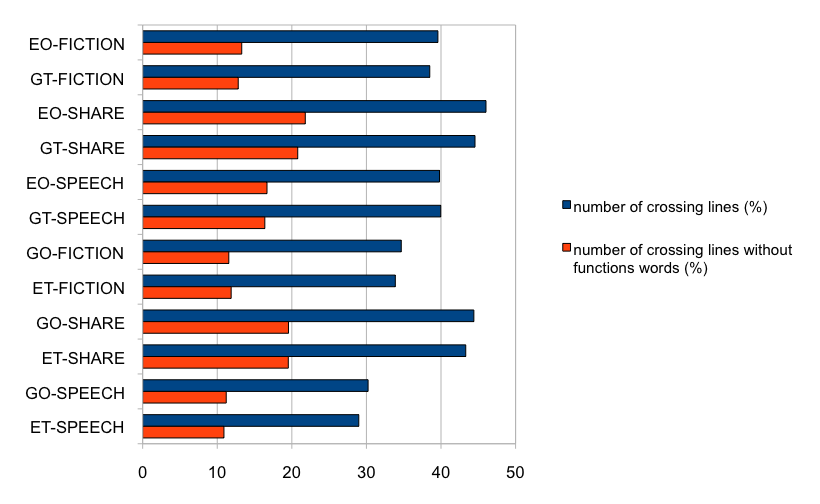
\includegraphics[width=\textwidth]{figures/CuloF5.png}
% \end{figure}

\begin{figure}
\begin{tikzpicture}

\begin{axis}[
    xbar,   % horizontal bars
    xmin=0, xmax=50,        % Start x axis at 0
     bar width=3pt,
    xlabel={Percentage (\%)},
    symbolic y coords={EO\_FICTION,GTrans\_FICTION,EO\_SHARE,GTrans\_SHARE,EO\_SPEECH,GTrans\_SPEECH,GO\_FICTION,ETrans\_FICTION,GO\_SHARE,ETrans\_SHARE,GO\_SPEECH,ETrans\_SPEECH},
    ytick=data,     % Use as many tick labels as y coordinates
    %yticklabels from table={\datatable}{Label},  % Get the labels from the Label column of the \datatable
    legend style={
            at={(1,.906)},
            anchor=east 
         	},
    reverse legend
]

% coordinates list is upside down, as
% algorithm seems to process last-in-first-out
\addplot [lsDarkBlue!80!black,fill=lsMidBlue] coordinates {           (10.9,ETrans\_SPEECH) (11.2,GO\_SPEECH)
(19.5,ETrans\_SHARE) (19.5,GO\_SHARE)
(11.9,ETrans\_FICTION) (11.5,GO\_FICTION)
(16.4,GTrans\_SPEECH) (16.7,EO\_SPEECH)
(20.8,GTrans\_SHARE) (21.8,EO\_SHARE)
(12.8,GTrans\_FICTION) (13.3,EO\_FICTION)};
\addplot [lsDarkBlue!80!black,fill=lsDarkBlue] coordinates {           (29.0,ETrans\_SPEECH) (30.2,GO\_SPEECH)
(43.3,ETrans\_SHARE) (44.4,GO\_SHARE)
(33.9,ETrans\_FICTION) (34.7,GO\_FICTION)
(40.0,GTrans\_SPEECH) (39.8,EO\_SPEECH)
(44.6,GTrans\_SHARE) (46.0,EO\_SHARE)
(38.5,GTrans\_FICTION) (39.6,EO\_FICTION)
};


\legend{Number of crossing lines,Number of crossing lines without function words}

\end{axis}

\end{tikzpicture}

\caption{Percentages of crossing lines between words and grammatical functions}
\label{fig:culo:5}
\end{figure}



This raises the question of why it is this level that appears to be prone to register influences. One starting point could be differing distributions of grammatical functions in the registers. If the grammatical functions are distributed differently in the four subcorpora in one register, this could be reflected in more crossing lines between originals and translations in this register. In order to assess the variation between subcorpora in the three registers, we compute the standard deviation between the values for each function in the individual registers. The sum of the individual standard deviations should be higher in a register containing more variation between the functions. As \tabref{tab:culo:3} shows, SHARE in fact has more variation reflected by higher standard deviations for the individual functions. The lowest variation is found in FICTION, which has consistently lower frequencies of crossing lines. 

\begin{table}
\small
\begin{tabular}{lrrrrr} 
\lsptoprule
& {FICTION}\\
\midrule
& EO & ETrans & GO & GTrans & Std. dev.\\
ADV\_* & 18.87 & 18.01 & 18.40 & 19.94 & 0.8335\\
APPO & 0.92 & 0.68 & 0.71 & 0.70 & 0.1141\\
COMPL & 5.19 & 5.04 & 3.78 & 3.28 & 0.9389\\
DOBJ & 10.77 & 10.26 & 10.82 & 11.76 & 0.6262\\
FIN & 23.43 & 23.20 & 24.39 & 23.87 & 0.5243\\
IOBJ & 0.81 & 0.81 & 1.93 & 2.03 & 0.6766\\
other & 6.76 & 7.61 & 7.75 & 7.09 & 0.4581\\
PRED & 6.04 & 6.75 & 4.83 & 5.26 & 0.8515\\
PROBJ & 1.74 & 1.75 & 2.49 & 2.27 & 0.3765\\
SUBJ & 21.08 & 21.27 & 19.86 & 19.37 & 0.9263\\
\midrule
& {SHARE}\\
\midrule
& EO & ETrans & GO & GTrans & Std. dev.\\
ADV\_* & 17.98 & 18.22 & 21.15 & 21.28 & 1.8005\\
APPO & 1.60 & 1.15 & 0.41 & 0.81 & 0.5065\\
COMPL & 6.42 & 6.54 & 4.16 & 4.15 & 1.3433\\
DOBJ & 12.19 & 10.73 & 10.47 & 11.54 & 0.7870\\
FIN & 22.54 & 21.75 & 20.96 & 21.33 & 0.6771\\
IOBJ & 0.88 & 0.93 & 1.70 & 1.54 & 0.4196\\
other & 11.07 & 12.10 & 12.64 & 11.50 & 0.6863\\
PRED & 7.22 & 9.12 & 8.87 & 8.27 & 0.8487\\
PROBJ & 2.84 & 2.62 & 4.40 & 4.68 & 1.0562\\
SUBJ & 21.32 & 20.82 & 19.78 & 19.17 & 0.9756\\
\midrule
& {SPEECH}\\
\midrule
& EO & ETrans & GO & GTrans & Std. dev.\\
ADV\_* & 14.61 & 15.52 & 16.91 & 15.90 & 0.9534\\
APPO & 0.81 & 1.41 & 0.83 & 0.42 & 0.4117\\
COMPL & 6.06 & 8.06 & 5.79 & 5.57 & 1.1422\\
DOBJ & 12.18 & 10.35 & 10.92 & 12.70 & 1.0893\\
FIN & 22.63 & 21.86 & 21.41 & 22.95 & 0.7017\\
IOBJ & 0.76 & 0.49 & 1.82 & 1.62 & 0.6467\\
OTHER & 6.79 & 7.96 & 9.05 & 6.30 & 1.2312\\
PRED & 11.08 & 10.21 & 8.27 & 8.92 & 1.2644\\
PROBJ & 2.93 & 2.21 & 3.94 & 4.25 & 0.9357\\
SUBJ & 22.05 & 21.85 & 21.00 & 21.24 & 0.4977\\
\lspbottomrule
\end{tabular}
\caption{Distribution of grammatical functions per subcorpus in percent}
\label{tab:culo:3}
\end{table}


While this appears to be a plausible explanation for the differing numbers of crossing lines, contrastive differences, i.e. an aspect not related to the register, could play a role as well. Prepositional objects and complements, for instance, display different frequencies in the two languages resulting in more similarities between originals and translations in the same language (see \tabref{tab:culo:3}). Apparently, prepositional objects play a greater role in the German registers whereas complements appear to be more typical of the English registers. Consequently, it is these functions in particular that seem to be more prone to crossing lines.

\tabref{tab:culo:4} displays the most frequent crossing lines between words and grammatical functions organized by register and translation direction. Due to the abovementioned weaknesses of recall in our word alignment, we do not interpret frequencies but only the ranking of the most common shifts. 

\begin{table}
\resizebox{\textwidth}{!}{
\begin{tabular}{llllll}
\lsptoprule
\multicolumn{2}{l}{FICTION} & \multicolumn{2}{l}{SHARE} & \multicolumn{2}{l}{SPEECH}\\
\midrule
E2G & G2E & E2G & G2E & E2G & G2E\\
dobj → subj & probj → dobj & compl → probj & probj → dobj & dobj → probj & subj → dobj\\
compl → dobj & dobj → subj & dobj → subj & subj → compl & dobj → compl & subj → compl\\
subj → dobj & fin → pred & dobj → probj & subj → dobj & compl → probj & probj → compl\\
dobj → fin & compl → subj & compl → dobj & probj → compl & subj → dobj & dobj → compl\\
dobj → probj & subj → dobj & dobj → compl & dobj → compl & dobj → subj & probj → dobj\\
fin → dobj & dobj → compl & compl → subj & fin → pred & pred → fin & dobj → subj\\
adv\_mod → dobj & fin → compl & probj → dobj & dobj → subj & compl → dobj & fin → compl\\
pred → fin & pred → fin & subj → dobj & compl → dobj & compl → subj & fin → pred\\
compl → subj & fin → subj & fin → pred & adv\_mod → compl & subj → compl & fin → subj\\
adv\_cause → dobj & fin → dobj & pred → fin & subj → probj & compl → fin & compl → subj\\
\lspbottomrule
\end{tabular}
}
\caption{The ten most frequent crossing lines per register and translation direction}
\label{tab:culo:4}
\end{table}


\tabref{tab:culo:4} shows how the translators shift from prepositional object to other functions in the translation direction German-English, thus adapting to the target language preferences, e.g. prepositional objects in the German FICTION texts are frequently translated by English direct objects. When translating from English to German, translators shift words away from complements to other functions, e.g. in SHARE to prepositional objects. \tabref{tab:culo:4} indicates that this also works in the opposite direction: translators not only avoid functions that are less typical in the target language, but also shift into preferred functions. Words are moved from various German functions into English complements, as exemplified by the second to fourth rank in SPEECH translations into English in \tabref{tab:culo:4}. A shift from German prepositional objects to English direct objects may be a general strategy not necessarily limited to a given register, as shown by the fact that this crossing line is most common in registers as divergent as FICTION and SHARE and is still fairly common in SPEECH. Examples \REF{ex:culo:19} to \REF{ex:culo:22} exemplify these shifts for the three registers.


\ea \label{ex:culo:19}
    \ea\label{ex:culo:verlassen} \textit{Er hat sich darauf verlassen, dass wir von drinnen sein Lächeln sehen können. }(GO\_FICTION\_007) 
    \ex \textit{He just assumed we could see his smile from inside.} (ETrans\_FICTION\_007) 
    \z
\z

Together with and initiated by the pronominal adverb \textit{darauf}, the whole \textit{dass }subordinate clause in the German original in \REF{ex:culo:19} forms a prepositional object. Note that the annotation on which this discussion is based is limited to the highest node in the sentence, thus the \textit{dass} clause is not analyzed further. This discontinuous prepositional object is shifted to a direct object in the English translation. In our query, the hit for the shift is triggered by the aligned noun pair \textit{Lächeln} in the German prepositional object and \textit{smile} in the English direct object. However, this analysis is somewhat problematic. Taking a closer look, we can see that \textit{Lächeln} is actually part of a direct object in the \textit{dass} clause, and should not account for the shift from prepositional object to the direct object. This effect is due to our top-level only annotation, an issue we will come back to in \sectref{sec:culo:5.2}.

\ea \label{ex:culo:20}
    \ea \textit{1995 haben wir auf 125 Jahre Deutsche Bank zurückgeblickt.} (GO\_SHARE\_009)\\
     \ex \textit{In 1995 we celebrated Deutsche Bank's 125th anniversary.} (ETrans\_SHARE\_009) 
     \z
\z
 
In \REF{ex:culo:20} from the SHARE register, the name of the bank reporting to its shareholders is shifted from the postmodification within the prepositional object in German to premodification of the direct object in the English translation. 

\ea \label{ex:culo:21}
  \ea \textit{Nach wie vor ist der Zinsüberschuß nach Risikovorsorge mit 9,7 Mrd DM die bei   weitem wichtigste Ertragskomponente. Allerdings weisen die unterschiedlichen   Steigerungsraten der einzelnen Ergebniskomponenten auf die Veränderungen im Geschäft hin. } (GO\_SHARE\_009)\\
   \ex \textit{Although net interest income after provision for losses on loans and advances, at DM 9.7 billion, is still by far the most important component of income, the individual figures highlight the changes in our business.} (ETrans\_SHARE\_009) 
   \z
\z


\ea \label{ex:culo:22}
   \ea \textit{Daher setzen wir uns nachdrücklich für die Schaffung eines europäischen Systems der Finanzaufsicht ein.} (GO\_SPEECH\_002) \\
    \ex \textit{Hence we expressly support the establishment of a European system of financial   supervision.} (ETrans\_SPEECH\_002) 
    \z
\z

Example \REF{ex:culo:21} still from SHARE and \REF{ex:culo:22} from SPEECH underline that the specific type of crossing lines exemplified there is largely due to lexical reasons. The German verb \textit{hinweisen} selects the preposition \textit{auf} for its object. Possibly, this finding points to a higher frequency of verbs taking certain types of prepositional object in German than in English. Globally, however, this has to be related to phrasal verbs whose particle is annotated as part of the verb in the CroCo annotation and consequently only leaving prepositional verbs as those taking a prepositional object. 

Other shifts may be more restricted to a given register, as, for instance, the shift from an English complement to a German prepositional object. This is particularly prominent in SHARE. Here, often similar reasons apply as with empty links for complements described in \sectref{sec:culo:4.1}.

Having established some potential causes for individual phenomena in the three registers, we can now return to the overall number of crossing lines on this level in the three registers. Compared to the other two registers under scrutiny here, the figures suggest that FICTION has relatively few crossing lines in both translation directions (see \figref{fig:culo:5}). Frequently, crossing lines concern changes between finite and predicator, as is the case in example (23). The perfect tense in the English original is translated by a present tense verb in German, thus resulting in a crossing line of \textit{happened} and \textit{geschieht}. 

\ea \label{ex:culo:23}
    \ea \textit{And what has happened before a few years have passed?} (EO\_FICTION\_006)\\
     \ex \textit{Und was geschieht, ehe noch ein paar Jahre vergangen sind?} (GTrans\_FICTION\_006) 
     \z
\z
 
 
While the shift in \REF{ex:culo:23} can be attributed to a deliberate change in tense by the translator, the shift between finite and predicator in \REF{ex:culo:24} is due to language contrast.

\ea\label{ex:culo:24}
  \ea 
\textit{Aber Sie wissen nichts. \textup{(GO\_FICTION\_007)}}\\
  \ex 
\textit{But you don't know anything. \textup{(ETrans\_FICTION\_007)}}
  \z
\z 


The English negation requires the auxiliary \textit{do} that results in the dissociation of the predicate into the finite auxiliary and the full verb as predicator. The German text does not require this and consequently only consists of a finite. 

An informationally more marked use of German as in \REF{ex:culo:25} results in a frequent crossing line in this register and translation direction, a shift between direct object and subject. 


\ea \label{ex:culo:25}
  \ea 
\textit{Die Frauen hat das nicht gerade zimperlich gemacht. \textup{(GO\_FICTION\_007)}}\\
   \ex \textit{The women weren't exactly prudes. \textup{(ETrans\_FICTION\_007)}}
   \z
\z

The translator has avoided putting the direct object at the front of the sentence in the English translation, as is the case in the German original. For English, this order of grammatical functions is highly marked. Preserving the order of the content, the translator here decided to shift \textit{women} to the subject function, adhering to the more rigid canonical order of grammatical functions in English, thus of course sacrificing some of the information structure of the original.

SPEECH contains the lowest number of crossing lines in the translation direction German to English. Even fairly complex structures as in \REF{ex:culo:26} do not necessarily require numerous shifts in grammatical functions.


\ea \label{ex:culo:26}
   \ea
\textit{Wenn wir also in diesem Sinne unseren Interessen und Werten dienen wollen, dann   muss Europa erstens wachsam gegenüber den neuen Bedrohungen sein, denen die   freien und offenen Gesellschaften ausgesetzt sind. \textup{(GO\_SPEECH\_010)}}\\
   \ex 
   \textit{So if we want to serve our interests and values in line with this definition, Europe must:   firstly, be vigilant to the new threats to which the free and open societies are exposed.   \textup{(ETrans\_SPEECH\_010)}}
   \z
\z

Possibly, this is due to a more canonical word order in the German SPEECH register requiring fewer adjustments in the English translation to conform to the more fixed word order of English. The percentage of subjects in sentence-initial position appears to corroborate this assumption. The percentages of grammatical subjects in relation to all grammatical functions in sentence-initial position in the German FICTION and SHARE registers are 42.16\% and 45.87\% respectively. By contrast, SPEECH exhibits 54.45\% of subjects in this position, displaying a register-specific feature and thus making the English translators' task easier.

In the opposite translation direction, SPEECH contains more crossing lines between words and grammatical functions. A potential language contrast between English and German is a shift from coordination to subordination as in \REF{ex:culo:27}. This is reflected in crossing lines because the whole subordinate clause in the translation is analyzed as one grammatical function in the CroCo annotation (here an adverbial) whereas the chunks in the coordinated clause are analyzed individually (\textit{resolution} is part of a direct object). 


\ea \label{ex:culo:27}
     \ea \textit{Every country has its own political issues and this makes resolution of our disputes increasingly difficult.} (EO\_SPEECH\_009)\\
      \ex \textit{Jedes Land hat seine eigenen politischen Anliegen, wodurch die Streitschlichtung zunehmend erschwert wird.} (GTrans\_SPEECH\_009) 
      \z
\z

Example \REF{ex:culo:28} displays a shift where the word \textit{fight} is moved from the direct object in the original to the subject in the German translation. This represents a typical case of modulation, where the perspective is shifted from the persons confronted with this fight to the fight itself. Beyond the translation shift of modulation this exemplifies \citegen{House1997} cross-cultural difference in terms of orientation towards persons in English versus orientation towards content in German. 

\ea \label{ex:culo:28}
   \ea \textit{And if the EU does as it has in the past, and provides financing to Airbus at below-  market rates of return, we could be facing a very large and highly contentious fight in the WTO.} (EO\_SPEECH\_009)\\
    \ex \textit{Und wenn die EU sich wie in der Vergangenheit verhält und dem Airbus Finanzierung zu Zinssätzen unter den auf dem Markt gültigen bietet, könnte uns ein großer und sehr kontroverser Kampf in der WTO bevorstehen.} (GTrans\_SPEECH\_009) 
    \z
\z

Word order contrasts combined with different mappings of semantic roles onto grammatical functions between English and German may typically result in crossing lines as represented by \REF{ex:culo:29}. The subject of the German passive original is positioned after the finite, which does not lead to an informationally highly marked construction in German. Rather than rearranging the linear precedence of clause elements in English, the translator has opted for rearranging the assignment of semantic roles to grammatical functions by choosing active voice. \textit{Basis}, the aligned translation of \textit{Grundlage}, is consequently no longer part of the subject but of the direct object. Example \REF{ex:culo:30} displays a similar case. 

\ea \label{ex:culo:29}
     \ea \textit{Gleichzeitig wurde hiermit auch die Grundlage für die Einführung von Hedgefonds in Deutschland und damit für den direkten Zugang deutscher Anleger zu diesem innovativen Produkt gelegt.} (GO\_SPEECH\_002)\\
      \ex \textit{At the same time it established the basis for the introduction of hedge funds in, thus affording German investors direct access to this innovative product.} (ETrans\_SPEECH\_002)
      \z
\z


\ea \label{ex:culo:30}
   \ea \textit{Damit werden Investitionen von rund 10 Mrd. DM angestoßen und 5--7 Mio. t CO2 eingespart.} (GO\_SPEECH\_001)\\
      \ex \textit{It will generate investments of around 10 billion marks and reduce CO2 emissions by 5--7 million metric tons.} (ETrans\_SPEECH\_001) 
      \z
\z

Examples \REF{ex:culo:31} and \REF{ex:culo:32} represent cases where there is no apparent reason forcing the translator to change the word order and, at the same time, the voice of the sentence. The crossing lines can be seen as symptoms of a whole range of changes that are obviously due to the translator. When seen in combination with the respective source sentence, these translations show clear indications of the translation process as a motivating variable. Nevertheless, they do not easily lend themselves to an interpretation in terms of translation properties as described by \citet{Baker1996} and others. 

\ea \label{ex:culo:31}
    \ea \textit{In Deutschland haben wir bisher noch keine Entscheidung über die Einführung von REITs getroffen. }(GO\_SPEECH\_002)\\
    \ex \textit{No decision has yet been taken in Germany on the introduction of REITs.} (ETrans\_SPEECH\_002) 
    \z
\z


\ea \label{ex:culo:32}
    \ea \textit{Dieser Markt hat sein Potenzial bei weitem noch nicht ausgeschöpft.} (GO\_SPEECH\_002)\\
     \ex \textit{The full potential of this market is by no means exhausted.} (ETrans\_SPEECH\_002)
     \z
\z

Concentrating on SHARE, where most of the crossing lines occur in both directions, we find examples like \REF{ex:culo:33}. Here, a different constituent structure (subject complement plus complementation in EO versus full verb plus prepositional object in GTrans) mapped onto very similar structures in terms of word order results in a crossing line. A certain share of instances of crossing lines can be analyzed in the same way. Example \REF{ex:culo:34}, however, is more representative of shifts occurring in translation in our data. Whereas \textit{Der Wandel} (\textit{the change}) constitutes the subject in the German original, it is realized as a prepositional object in the translation with the patient becoming the subject. This results in a major shift in perspective in the translation. 

\ea \label{ex:culo:33}
    \ea \textit{The same is true for Human Resources reviews.} (EO\_SHARE\_004)\\
    \ex \textit{Das gleiche gilt für ``Human Resources Reviews''.} (GTrans\_SHARE\_004) 
    \z
\z


\ea \label{ex:culo:34}
    \ea \textit{Der Wandel geht an unseren Filialen nicht vorüber.} (GO\_SHARE\_009)\\
    \ex \textit{Our branches are not unaffected by these changes.} (ETrans\_SHARE\_009) 
    \z
\z
 
The crossing line in example \REF{ex:culo:35} is equally interesting in that, among a number of shifts, the subject of the original (\textit{die moderne Universalbank}) is hidden in the postmodification of the complement in the translation (\textit{an impressive demonstration of a modern universal bank's capabilities}). 

\ea \label{ex:culo:35}
     \ea \textit{Mit ihrer Plazierungskraft im Inland hat die moderne Universalbank ihre Möglichkeiten eindrucksvoll unterstrichen.} (GO\_SHARE\_009)\\
     \ex \textit{The placement of this issue in Germany was an impressive demonstration of a modern   universal bank's capabilities.} (ETrans\_SHARE\_009)
     \z
\z

Beyond modulation as a type of translation shift these crossing lines do not easily lend themselves to interpretations in terms of translation properties. Instances like \REF{ex:culo:35} point to implicitation rather than explicitation in terms of constituency structure, because the referent (and the words) contained in the subject in the original is not only shifted into the complement in the translation, but is additionally reduced to postmodification instead of representing the head of the phrase in the original.

The discussion of crossing lines between words and grammatical functions has shown that these crossing lines are symptomatic of a whole range of factors relevant to translation. Of course they are subject to a wide range of influences that prohibit mono-causal explanations. They are, however, indicative of differences between registers as well as contrastive differences in the frequency of certain grammatical functions and in word order. Furthermore, they show translation shifts, typically in the area of modulation, which must often be attributed to translator behavior. Finally, we have also shown dimensions of cross-cultural differences in House's sense at work.

A direct and simplistic association between crossing lines between words and grammatical functions and translation properties should be avoided: while crossing lines definitely have implications for properties such as explicitation, normalization, simplification, shining through and others, the relationship is complex and needs further evidence.


\section{Future work}\label{sec:culo:5}

We have shown in this paper the query power which can be provided by an annotation which comprises multi-level annotation and alignment and which to a considerable extent can be done (semi-)automatically, at least when it comes to tagging and chunking. The value of the CroCo-specific annotation lies on the one hand in the alignment which was partly done by human annotators (for the clause and sentence level). On the other hand, the manual annotation of levels like phrase structure and grammatical functions delivers a high-quality set of data. Moreover, we have demonstrated the methodological value of querying empty links and crossing lines for the detection of translation shifts and investigation of translation properties. Within the context of the CroCo project there are a number of spin-off projects, e.g. further investigating cohesion in originals and translations, or how ``parallel'' valency is between English and German. In some of these projects, the limitations of the CroCo annotation -- esp. the decision to keep the functional annotation on the top level, with the exception of clauses which are annotated for their functions as well -- become obvious.

In \sectref{sec:culo:5.1} we outline some thoughts on how the findings in this paper will help realize a project on valency queries. In order to study valency and other phenomena in a more detailed fashion and on all linguistic levels, i.e. with respect not just to main and subordinate clauses, but also to embedded structures, we will add deeper annotation levels to CroCo. We briefly sketch out these plans in \sectref{sec:culo:5.2}.

\subsection{Valency queries}\label{sec:culo:5.1}

One of the big hopes in parallel corpora is that they may enable us to build multilingual valency dictionaries (semi-)automatically. This would facilitate the work of the lexicographer enormously. Corpora allow for the extraction of large amounts of data in a short time and may contain examples a lexicographer would not easily think of. Examples for monolingual valency dictionaries based on corpora are the Czech PDT-VALLEX\footnote{http://ufal.mff.cuni.cz/vallex/2.5/doc/home.html} and the English Erlangen Valency Pattern Bank.\footnote{http://www.patternbank.uni-erlangen.de/cgi-bin/patternbank.cgi}

In order for valency queries to work, we must rely on the fact that the structures are maximally equivalent between original and translation. As we have seen in our results, this is more valid for some linguistic levels than for others. For the sentence level, for instance, we found that in all registers and all translation directions at least 99\% of the sentences have an equivalent. If we see the sentence as a valency carrier plus the complements and adjuncts accompanying it, this means for the purpose of valency extraction that in 99\% of all cases we will have a pair of structures which can be used for further investigation.


The results on empty links and crossing lines for grammatical functions, which we presented in this paper, will be most valuable for our valency studies as well. The considerable number of occurrences for these two phenomena already suggest that we are likely to find quite a number of valency-related phenomena which occur in translation. In example \REF{ex:culo:12}, for instance, we have a case in which the nominal group \textit{zur Sicherung von Beschäftigung} was translated with a verbal expression \textit{to safeguarding jobs}, resulting in an empty link on the clause level. From a valency point of view, the shift from noun to verb also shifts the syntactic valency frame of \textit{Sicherung} which adds the object as a \textit{von}{}-PP, compared to the direct object \textit{jobs} that the verbal equivalent \textit{safeguarding} requires. Another kind of valency shift involves cases of shifts in grammatical functions, which have been described in \sectref{sec:culo:4.3}. Furthermore, a pilot study has revealed that there is a considerable percentage of cases in which the main verbs do not perfectly match. This was the case for about 20-40\% in our sample of 300 sentence pairs (50 from each register and translation direction). For the instances of divergences found, there was either a shift in meaning (e.g. \textit{jmdm. gut tun} `do so. good' vs. \textit{benefit from sth.}) or the full verb on the one side has a syntactically more complex equivalent on the other side, e.g. a copula construction, an idiomatic expression or a support verb construction, often changing the overall structure of the sentence. As for copula constructions, it has already been outlined in \sectref{sec:culo:4.1} that they are more frequent in English and thus account for quite a number of empty links for shifts departing from (predicative) complements. There seems to be only a small minority of cases in which a sentence has been completely re-phrased, thus rendering the sentence pair useless for the study of valency-related phenomena.

In order to study these phenomena, we will need a deeper annotation of structures, which will be provided by converting (parts of) the CroCo corpus to a parallel dependency treebank, the plans for which are briefly outlined in the following subsection.

\subsection{Towards a parallel treebank}\label{sec:culo:5.2}

Let us go back to our \textit{Lächeln}-example \REF{ex:culo:19} from \sectref{sec:culo:4.3}. We can see in this example, as has already been discussed in \sectref{sec:culo:4.3}, that the top-level-only annotation in CroCo sometimes negatively affects our queries. The \textit{dass}-clause is combined into a prepositional object together with the \textit{darauf}-adverb. When querying for the word pair \textit{Lächeln} and \textit{smile}, we get a shift from prepositional object to direct object, which is triggered by our method of analyzing the structure rather than a real shift. This kind of annotation is also disadvantageous when looking into valency phenomena. Elements might be deeper embedded when shifting from full verb to copula plus adjective-constructions, for instance. We would like to be able to detect these kinds of shifts automatically as well.

We have thus decided to transform at least parts of the CroCo-annotation into a parallel dependency treebank, in a spin-off project. When tentatively translating our functional analysis of the German original sentence from the \textit{Lächeln}-example into a dependency tree, we could get an analysis as exemplified in \figref{fig:culo:6}. From a dependency tree like that depicted in the figure, we can deduce the correct grammatical function for \textit{Lächeln}, but still preserve the information that the whole subordinate clause with \textit{sehen} as root functions as a prepositional object.

\begin{figure} 
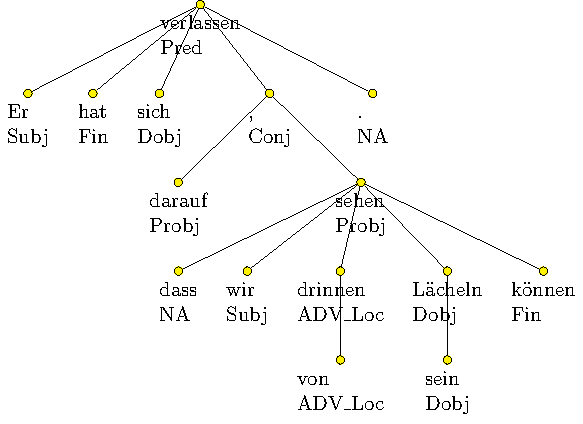
\includegraphics[width=\textwidth]{figures/CuloF6.pdf}
\caption{A possible dependency analysis for example \REF{ex:culo:verlassen}}
\label{fig:culo:6}
\end{figure}


We will be using the tools created within the Prague Dependency Treebank project, namely TrEd\footnote{\url{http://ufal.mff.cuni.cz/~pajas/tred/}} plus some extensions for working with parallel data which it delivers \citep{BöhmováEtAl2000}. We will annotate dependencies at the functional level, using grammatical categories such as subject, object etc. Annotation of deep syntactic or semantic roles is not planned at present, but may be added at a later stage. The trees will be aligned on the level of the grammatical functions. This alignment will allow us to more reliably query shifts on this level.



{\sloppy 
\printbibliography[heading=subbibliography,notkeyword=this]
}
\end{document}

